\subsection{Momentum Avanzado y Reducción de Varianza (2024--2025)}
\paragraph{Adan (Momentum Nesterov Adaptativo).}
\begin{figure}[H]
\centering
\fitfigure{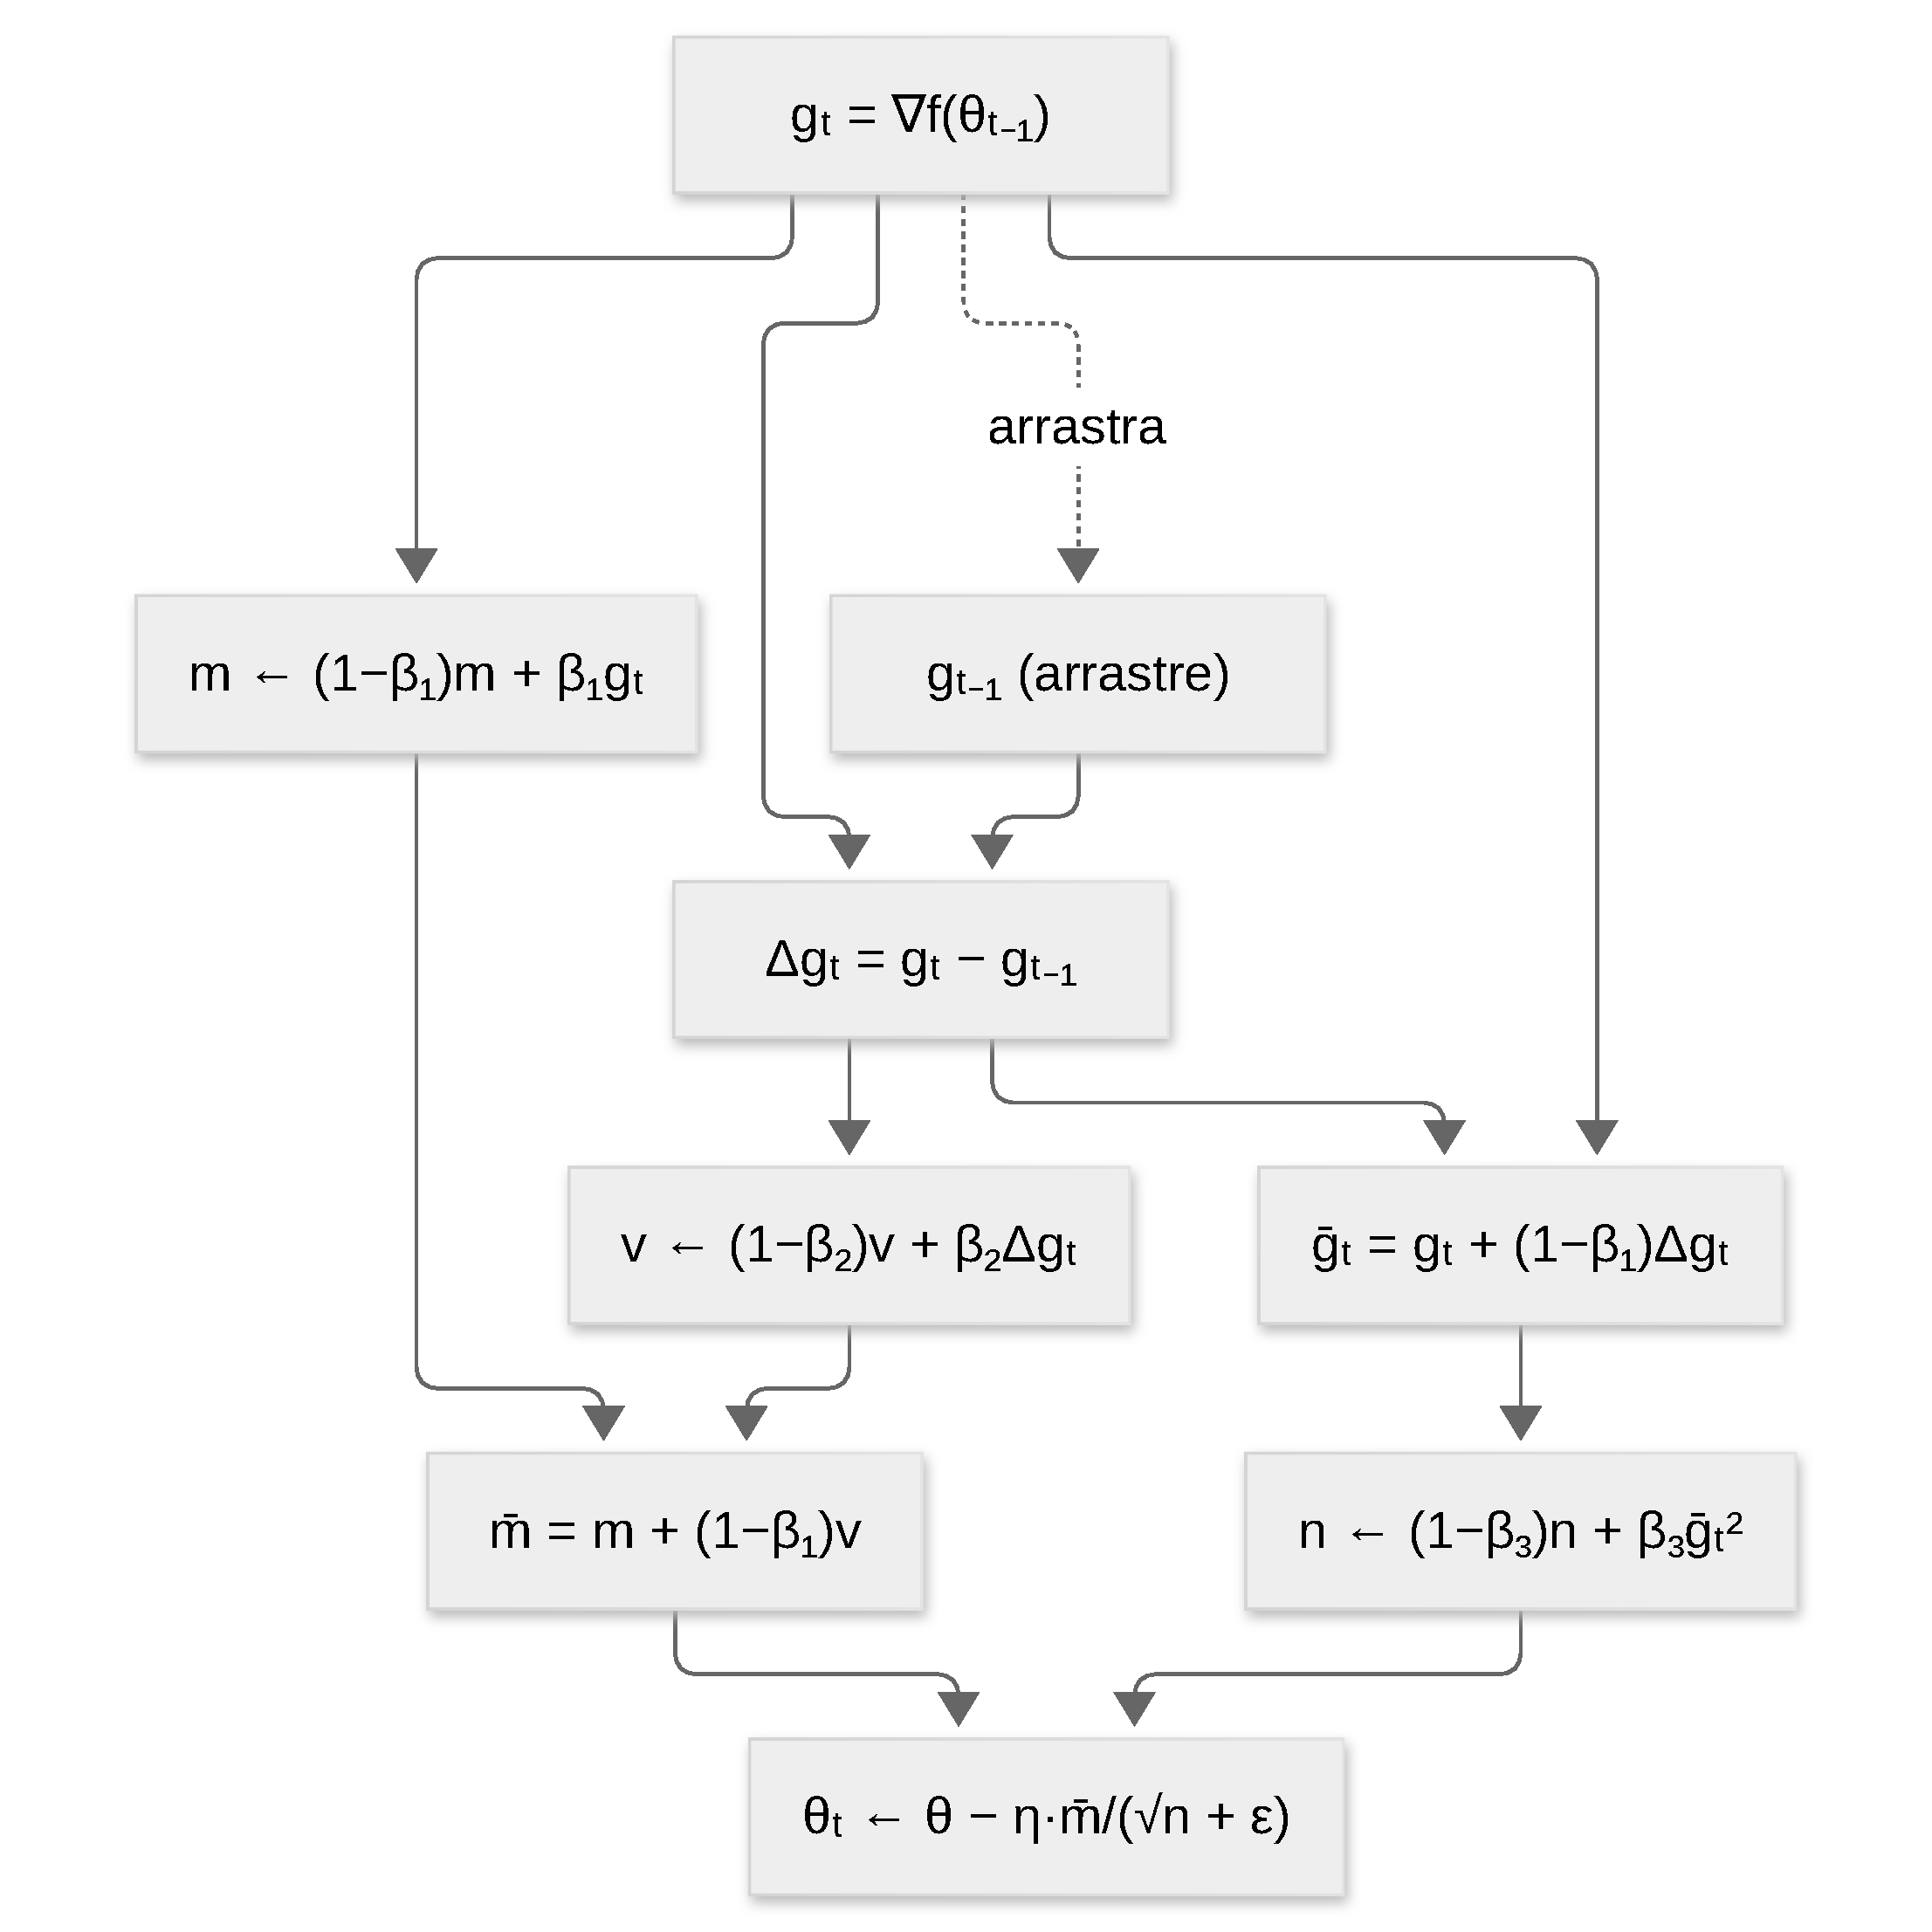
\includegraphics{../paper/figures/optimizers/adan-es.pdf}}
\caption{Flujo por paso de Adan: estimación de momentum de Nesterov a partir de la diferencia de gradientes, con tres búferes de estado y un paso de momentum combinado.}
\label{fig:opt-adan}
\end{figure}
Adan reformula la aceleración de Nesterov sin el cálculo de gradiente adicional requerido por el SGD Nesterov clásico. El algoritmo mantiene tres búferes de momentum:
\begin{align}
m_t &= (1-\beta_1)m_{t-1} + \beta_1 g_t \quad\text{(primer momento)} \\
v_t &= (1-\beta_2)v_{t-1} + \beta_2(g_t - g_{t-1}) \quad\text{(velocidad/diferencia de gradientes)} \\
n_t &= (1-\beta_3)n_{t-1} + \beta_3[g_t + (1-\beta_1)(g_t-g_{t-1})]^2 \quad\text{(segundo momento Nesterov)}
\end{align}
El término de \textbf{Estimación de Momentum Nesterov} (NME) $\bar{g}_t = g_t + (1-\beta_1)(g_t-g_{t-1})$ estima el gradiente en una posición futura sin evaluarlo. La actualización combina el momentum con la velocidad:
\[\bar{m}_t = m_t + (1-\beta_1)v_t, \quad \theta_{t+1} = \theta_t - \eta\frac{\bar{m}_t}{\sqrt{n_t}+\epsilon}\]

\begin{algorithm}[H]
\caption{Adan (Momentum Nesterov Adaptativo)}
\label{alg:adan}
\begin{algorithmic}[1]
\Require Parámetros iniciales $\theta_0$, tasa de aprendizaje $\eta$, $\beta_1, \beta_2, \beta_3 \in (0,1)$
\Ensure Parámetros actualizados $\theta_T$
\State Inicializar: $m \gets 0$, $v \gets 0$, $n \gets 0$, $g_{-1} \gets 0$ (gradiente anterior)
\For{$t = 1, 2, \ldots, T$}
    \State $g_t \gets \nabla f(\theta_{t-1})$
    \State $m \gets (1-\beta_1) m + \beta_1 g_t$
    \State $\Delta g_t \gets g_t - g_{t-1}$
    \State $v \gets (1-\beta_2) v + \beta_2 \Delta g_t$
    \State Estimación Nesterov: $\bar{g}_t \gets g_t + (1-\beta_1) \Delta g_t$
    \State $n \gets (1-\beta_3) n + \beta_3 \bar{g}_t^2$
    \State Momentum combinado: $\bar{m} \gets m + (1-\beta_1) v$
    \State $\theta_t \gets \theta_{t-1} - \eta (\bar{m} / (\sqrt{n} + \epsilon))$
    \State $g_{t-1} \gets g_t$
\EndFor
\Return $\theta_T$
\end{algorithmic}
\end{algorithm}

\paragraph{Contras.}
\begin{itemize}[leftmargin=*]
\item Tres búferes tipo momentum aumentan la sobrecarga de memoria respecto a Adam.
\item Contabilidad adicional de la diferencia de gradientes en cada paso.
\end{itemize}

\paragraph{Ventajas.}
\begin{itemize}[leftmargin=*]
\item Aceleración estilo Nesterov sin una evaluación adicional del gradiente.
\item Convergencia rápida en arquitecturas diversas (CNN, GAN, transformadores).
\end{itemize}

\paragraph{ADOPT (Adam con Ajuste Óptimo Podado).}
\begin{figure}[H]
\centering
\fitfigure{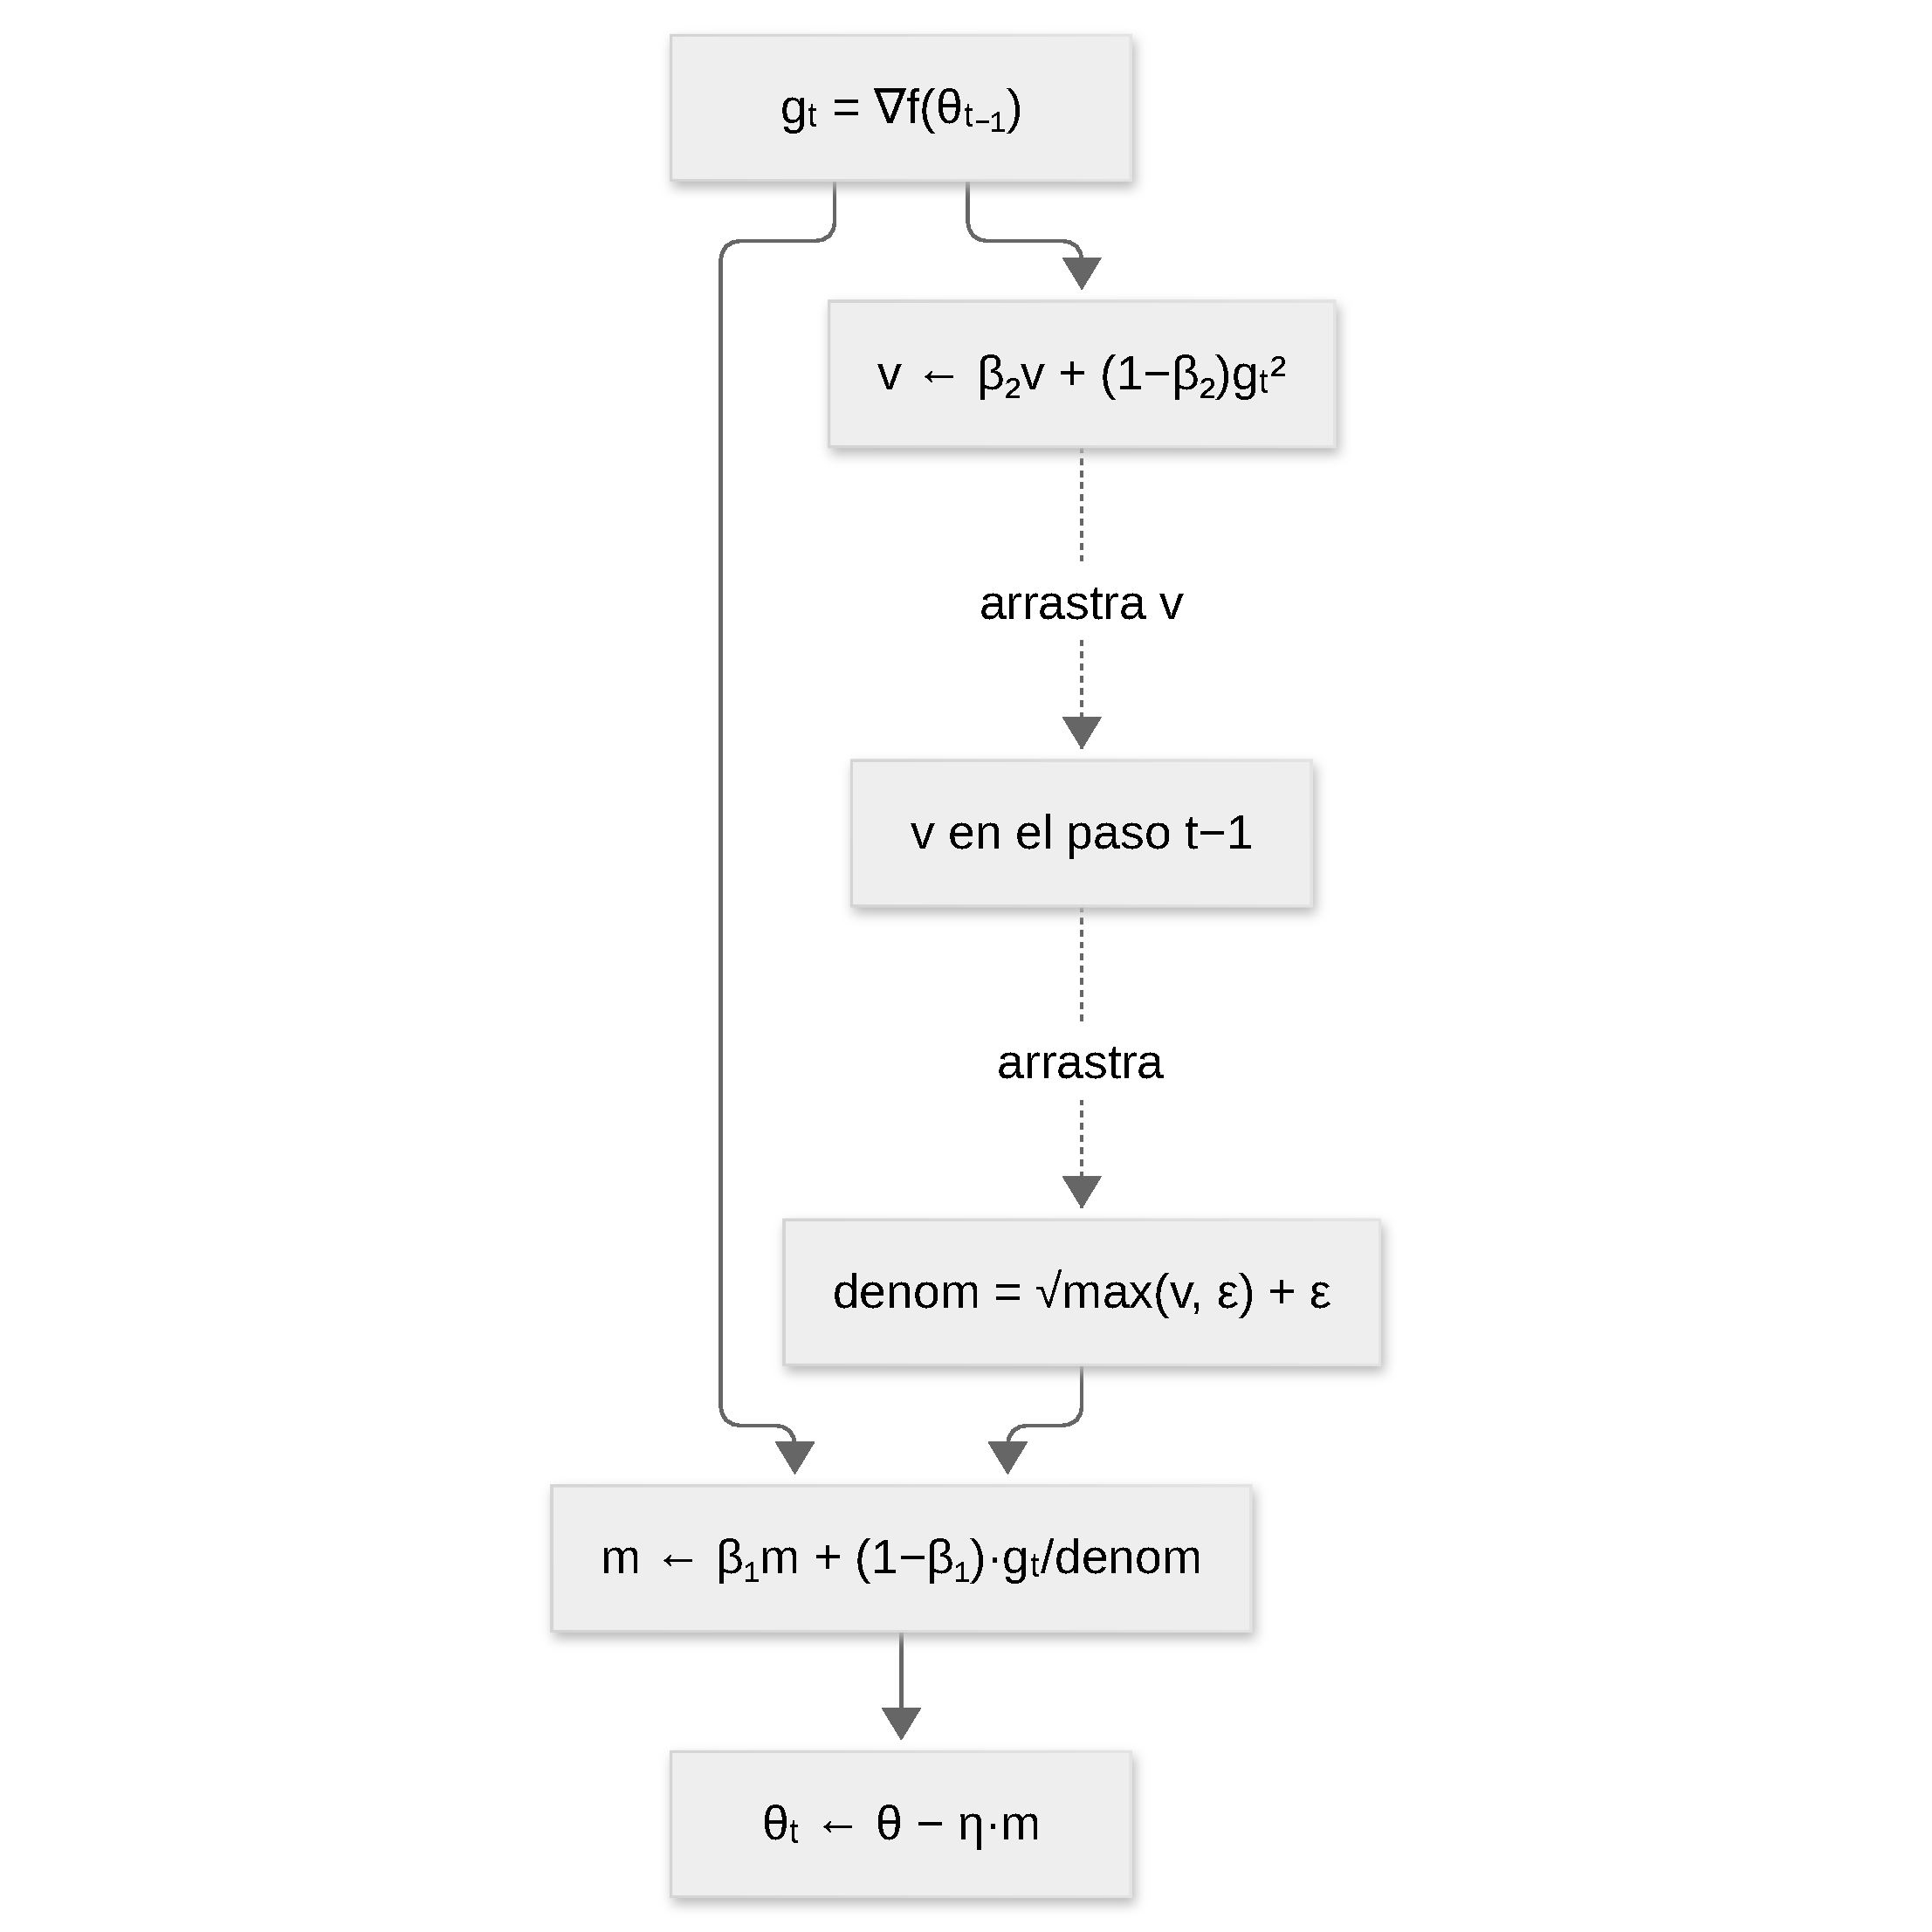
\includegraphics{../paper/figures/optimizers/adopt-es.pdf}}
\caption{Flujo por paso de ADOPT: el segundo momento del paso anterior normaliza el gradiente actual antes de actualizar el primer momento.}
\label{fig:opt-adopt}
\end{figure}
ADOPT corrige un problema teórico fundamental en Adam: el gradiente aparece tanto en la estimación del primer momento como en la del segundo momento, creando circularidad. ADOPT \textbf{desacopla} utilizando el segundo momento del paso anterior para el denominador:
\begin{align}
v_t &= \beta_2 v_{t-1} + (1-\beta_2)g_t^2 \\
m_t &= \beta_1 m_{t-1} + (1-\beta_1)\frac{g_t}{\sqrt{v_{t-1}}+\epsilon} \quad\text{(usa $v_{t-1}$, no $v_t$)} \\
\theta_{t+1} &= \theta_t - \eta m_t
\end{align}

\begin{algorithm}[H]
\caption{ADOPT (Adam con Ajuste Óptimo Podado)}
\label{alg:adopt}
\begin{algorithmic}[1]
\Require Parámetros iniciales $\theta_0$, tasa de aprendizaje $\eta$, $\beta_1, \beta_2$, tolerancia $\epsilon$
\Ensure Parámetros actualizados $\theta_T$
\State Inicializar: $m \gets 0$, $v \gets 0$
\For{$t = 1, 2, \ldots, T$}
    \State $g_t \gets \nabla f(\theta_{t-1})$
    \If{decadencia\_de\_peso $> 0$}
        \State $\theta_{t-1} \gets \theta_{t-1}(1 - \eta\lambda)$
    \EndIf
    \State Usar segundo momento \textbf{anterior}: $\text{denom} \gets \sqrt{\max(v, \epsilon)} + \epsilon$
    \State Actualizar primer momento usando varianza anterior: $m \gets \beta_1 m + (1-\beta_1)(g_t / \text{denom})$
    \State Actualizar segundo momento con gradiente \textbf{actual}: $v \gets \beta_2 v + (1-\beta_2) g_t^2$
    \State $\theta_t \gets \theta_{t-1} - \eta m$
\EndFor
\Return $\theta_T$
\end{algorithmic}
\end{algorithm}

\paragraph{Contras.}
\begin{itemize}[leftmargin=*]
\item Requiere conservar el segundo momento anterior como denominador explícito.
\item Las ganancias empíricas dependen de la arquitectura y del ajuste.
\end{itemize}

\paragraph{Ventajas.}
\begin{itemize}[leftmargin=*]
\item Elimina la circularidad del gradiente de Adam y alcanza la tasa óptima $O(1/\sqrt{T})$ con \textbf{cualquier} $\beta_2 \in (0,1)$, sin suposiciones de ruido acotado.
\item Reemplazo directo de Adam con rendimiento empírico comparable o superior en visión, PLN, RL y modelado generativo.
\end{itemize}

\paragraph{AdEMAMix (Mezcla de Promedios Móviles Exponenciales).}
\begin{figure}[H]
\centering
\fitfigure{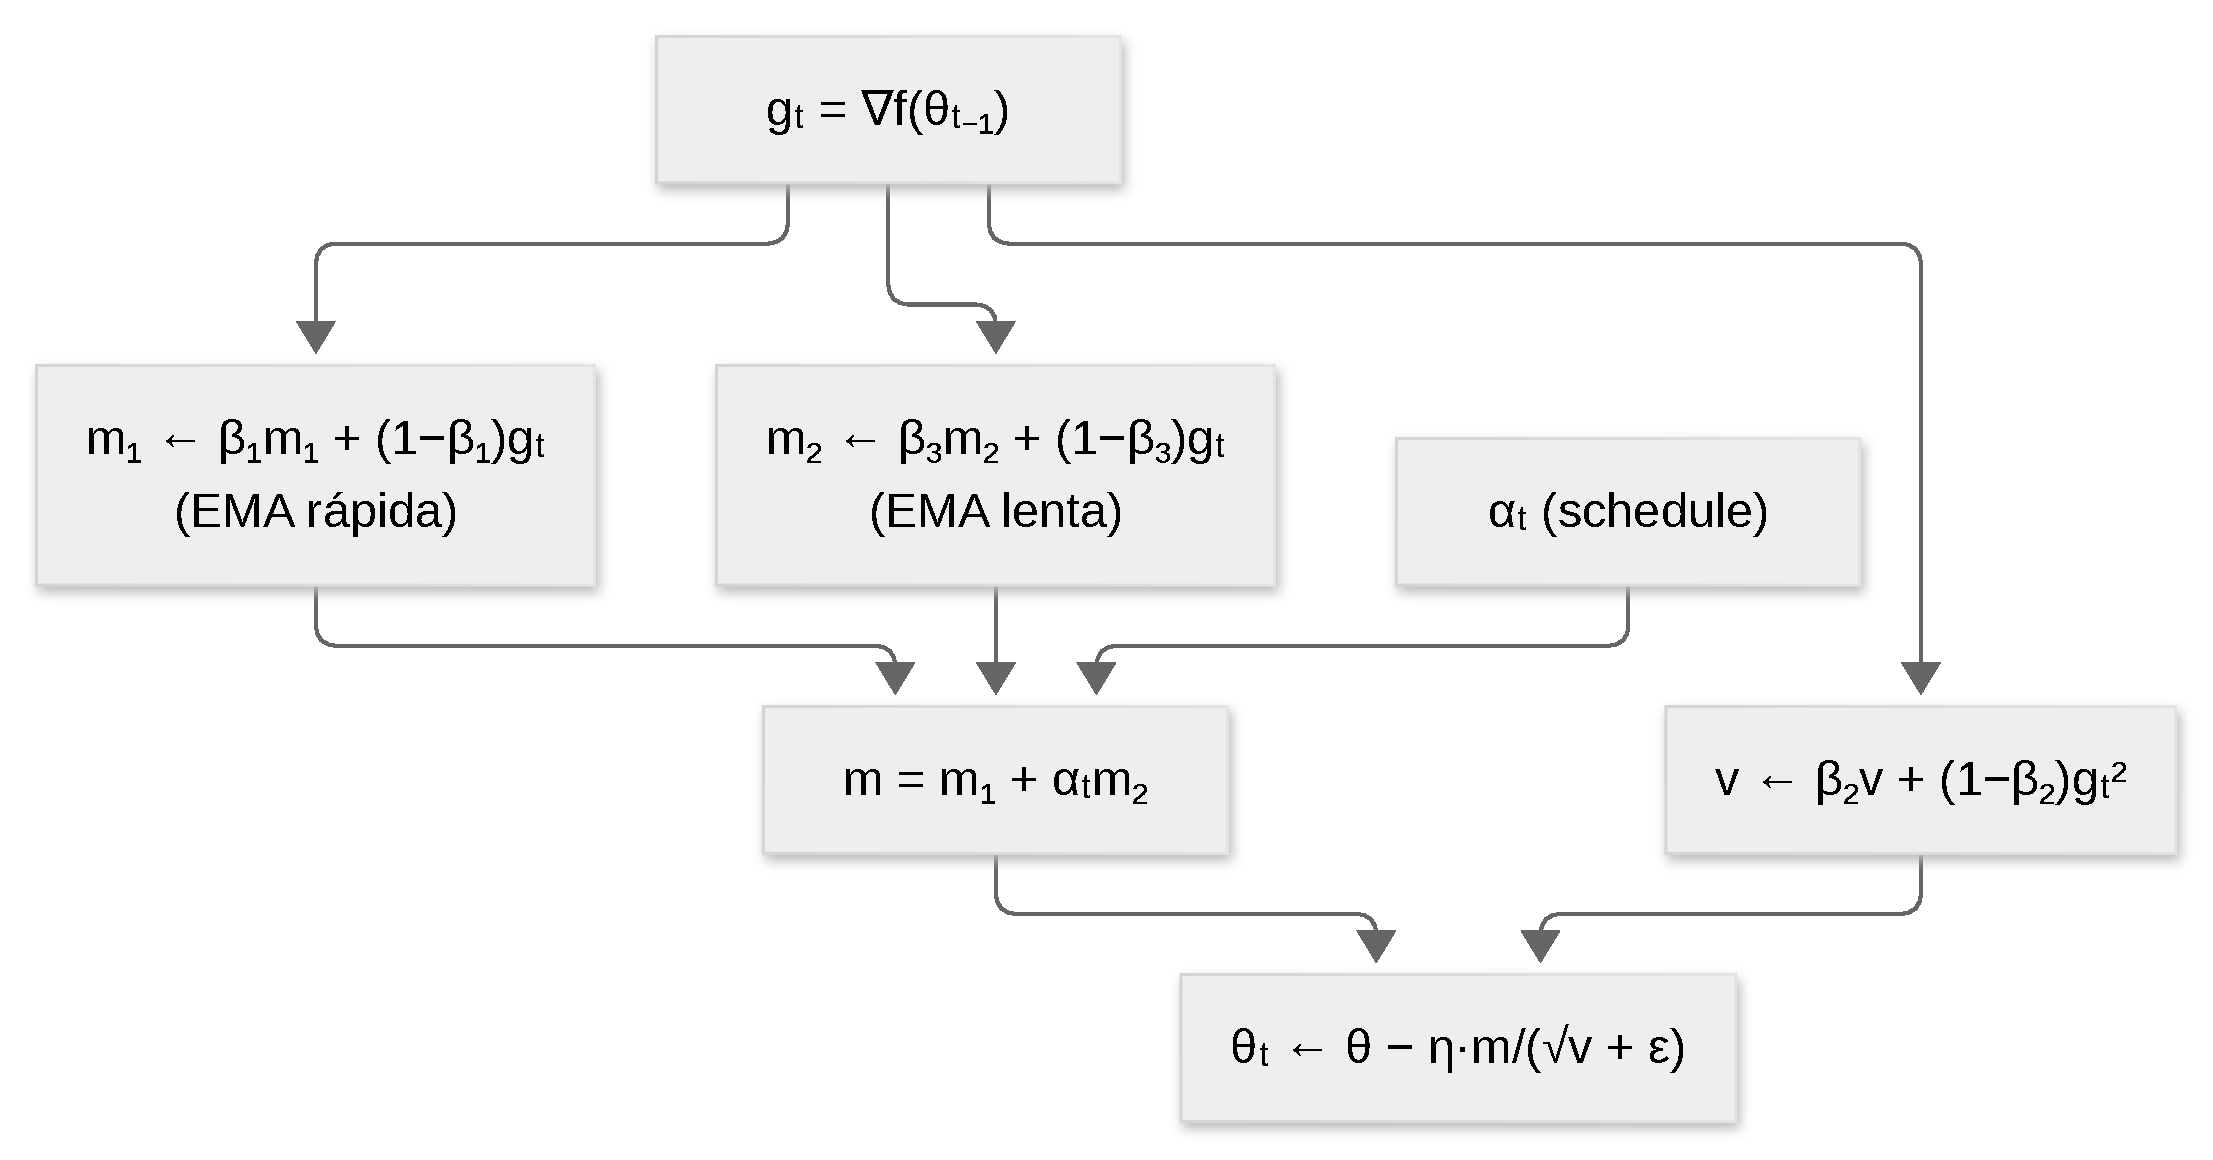
\includegraphics{../paper/figures/optimizers/ademamix-es.pdf}}
\caption{Flujo por paso de AdEMAMix: EMAs rápida y lenta en paralelo, mezcladas con un peso programado $\alpha_t$ antes de la actualización adaptativa.}
\label{fig:opt-ademamix}
\end{figure}
AdEMAMix reemplaza el EMA único de gradientes de Adam por una \textbf{mezcla de dos EMA}: uno de decadencia rápida y otro de decadencia lenta. Esto aborda la observación de que los gradientes siguen siendo informativos durante decenas de miles de pasos, no solo cientos:
\begin{align}
m_{1,t} &= \beta_1 m_{1,t-1} + (1-\beta_1)g_t \quad\text{(EMA rápido, $\beta_1 \approx 0.9$)} \\
m_{2,t} &= \beta_3 m_{2,t-1} + (1-\beta_3)g_t \quad\text{(EMA lento, $\beta_3 \approx 0.9999$)} \\
v_t &= \beta_2 v_{t-1} + (1-\beta_2)g_t^2 \\
m_t &= m_{1,t} + \alpha_t m_{2,t} \quad\text{(mezcla con peso programado $\alpha_t$)} \\
\theta_{t+1} &= \theta_t - \eta\frac{m_t}{\sqrt{v_t}+\epsilon}
\end{align}
El peso de la mezcla $\alpha_t$ típicamente aumenta durante el entrenamiento, permitiendo que el EMA rápido proporcione adaptación inmediata mientras que el EMA lento acumula correlaciones de gradiente a largo plazo.

\begin{algorithm}[H]
\caption{AdEMAMix (Mezcla de Promedios Móviles Exponenciales)}
\label{alg:ademamix}
\begin{algorithmic}[1]
\Require Parámetros iniciales $\theta_0$, tasa de aprendizaje $\eta$, $\beta_1$ (rápido), $\beta_3$ (lento), $\beta_2$ (segundo momento)
\Require Peso de mezcla $\alpha_t$ (típicamente creciente), tolerancia $\epsilon$
\Ensure Parámetros actualizados $\theta_T$
\State Inicializar: $m_1 \gets 0$ (EMA rápido), $m_2 \gets 0$ (EMA lento), $v \gets 0$
\For{$t = 1, 2, \ldots, T$}
    \State $g_t \gets \nabla f(\theta_{t-1})$
    \If{decadencia\_de\_peso $> 0$}
        \State $\theta_{t-1} \gets \theta_{t-1}(1 - \eta\lambda)$
    \EndIf
    \State $m_1 \gets \beta_1 m_1 + (1-\beta_1) g_t$ \Comment{EMA rápido}
    \State $m_2 \gets \beta_3 m_2 + (1-\beta_3) g_t$ \Comment{EMA lento}
    \State $v \gets \beta_2 v + (1-\beta_2) g_t^2$
    \State $m_t \gets m_1 + \alpha_t m_2$ \Comment{Mezcla}
    \State $\theta_t \gets \theta_{t-1} - \eta (m_t / (\sqrt{v} + \epsilon))$
\EndFor
\Return $\theta_T$
\end{algorithmic}
\end{algorithm}

\paragraph{Contras.}
\begin{itemize}[leftmargin=*]
\item Dos EMA de gradiente más el segundo momento casi triplican el estado del optimizador de Adam.
\item La programación de mezcla $\alpha_t$ añade un hiperparámetro que ajustar.
\end{itemize}

\paragraph{Ventajas.}
\begin{itemize}[leftmargin=*]
\item Explota información de gradiente que sigue siendo informativa durante decenas de miles de pasos.
\item Un modelo de 1.3B en 101B tokens iguala a AdamW en 197B tokens (ganancia del 95\% en eficiencia de datos), lo que sugiere menor olvido.
\end{itemize}

\paragraph{MARS (Haciendo Brillar las Tasas de Aprendizaje Adaptativas).}
\begin{figure}[H]
\centering
\fitfigure{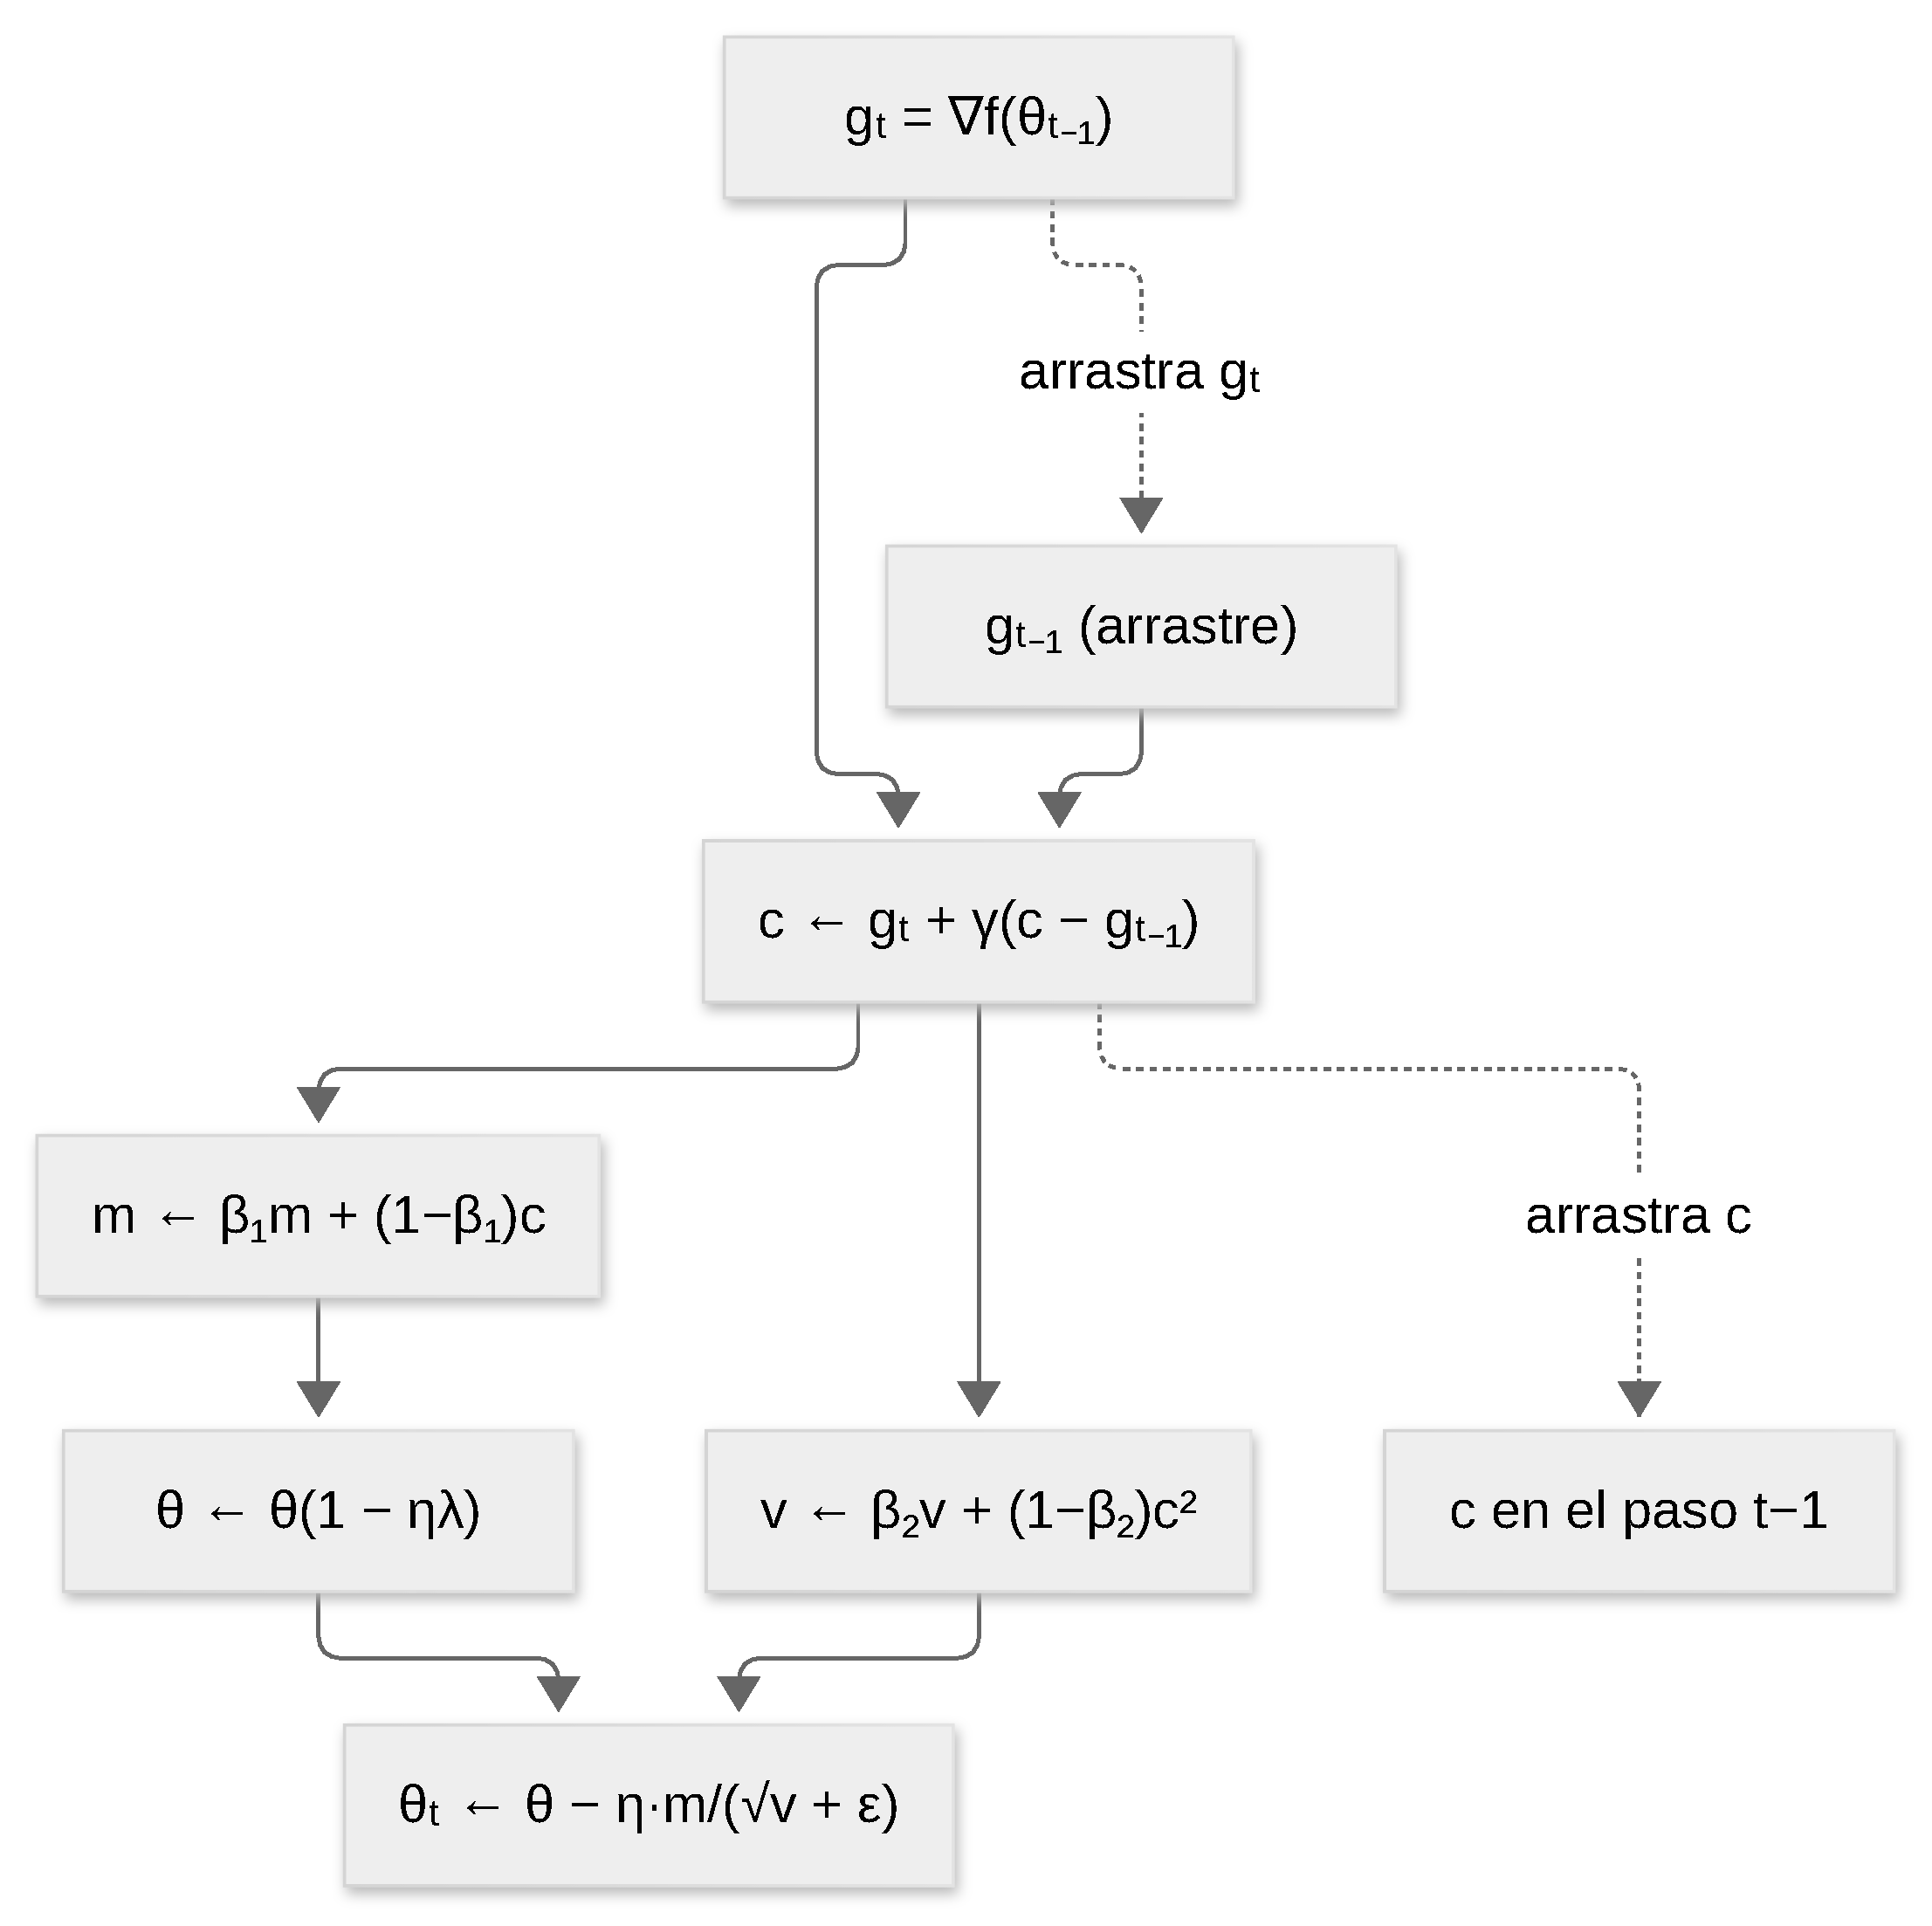
\includegraphics{../paper/figures/optimizers/mars-es.pdf}}
\caption{Flujo por paso de MARS: una estimación recursiva de gradiente con varianza reducida que alimenta los momentos de primer y segundo orden estilo Adam.}
\label{fig:opt-mars}
\end{figure}
MARS combina métodos de gradiente precondicionado (ej., AdamW) con \textbf{reducción de varianza} mediante momentum recursivo estocástico escalado. La innovación central es una estimación del gradiente con varianza reducida:
\begin{align}
c_t &= g_t + \gamma(c_{t-1} - g_{t-1}) \quad\text{(estimación recursiva tipo SVRG)} \\
m_t &= \beta_1 m_{t-1} + (1-\beta_1)c_t \\
v_t &= \beta_2 v_{t-1} + (1-\beta_2)c_t^2 \\
\theta_{t+1} &= \theta_t - \eta\frac{m_t}{\sqrt{v_t}+\epsilon}
\end{align}
donde $\gamma \in [0.01, 0.1]$ controla cuánta información de gradiente histórico se retiene. El gradiente con varianza reducida $c_t$ actúa como un filtro de ruido implícito, amplificando las direcciones de señal consistentes y amortiguando el ruido contradictorio.

\begin{algorithm}[H]
\caption{MARS (Haciendo Brillar las Tasas de Aprendizaje Adaptativas)}
\label{alg:mars}
\begin{algorithmic}[1]
\Require Parámetros iniciales $\theta_0$, tasa de aprendizaje $\eta$, $\beta_1, \beta_2$, decadencia de peso $\lambda$
\Require Coeficiente de reducción de varianza $\gamma \in [0.01, 0.1]$
\Ensure Parámetros actualizados $\theta_T$
\State Inicializar: $m \gets 0$, $v \gets 0$, $c \gets 0$ (gradiente con varianza reducida), $g_{-1} \gets 0$
\For{$t = 1, 2, \ldots, T$}
    \State $g_t \gets \nabla f(\theta_{t-1})$
    \State Reducción de varianza: $c \gets g_t + \gamma(c - g_{t-1})$
    \State $m \gets \beta_1 m + (1-\beta_1) c$
    \State $v \gets \beta_2 v + (1-\beta_2) c^2$
    \If{decadencia\_de\_peso $> 0$}
        \State $\theta_{t-1} \gets \theta_{t-1}(1 - \eta\lambda)$
    \EndIf
    \State $\theta_t \gets \theta_{t-1} - \eta (m / (\sqrt{v} + \epsilon))$
    \State $g_{t-1} \gets g_t$
\EndFor
\Return $\theta_T$
\end{algorithmic}
\end{algorithm}

\paragraph{Contras.}
\begin{itemize}[leftmargin=*]
\item Almacena el gradiente con varianza reducida y el gradiente anterior además de los momentos de Adam.
\item El coeficiente de reducción de varianza $\gamma \in [0.01, 0.1]$ debe ajustarse.
\end{itemize}

\paragraph{Ventajas.}
\begin{itemize}[leftmargin=*]
\item Actúa como un filtro de ruido implícito, amplificando direcciones consistentes y amortiguando el ruido contradictorio.
\item MARS-AdamW supera consistentemente a AdamW por márgenes significativos en el preentrenamiento de GPT-2.
\end{itemize}

\paragraph{Optimizadores Cautelosos (Cautious AdamW, Cautious Lion).}
\begin{figure}[H]
\centering
\fitfigure{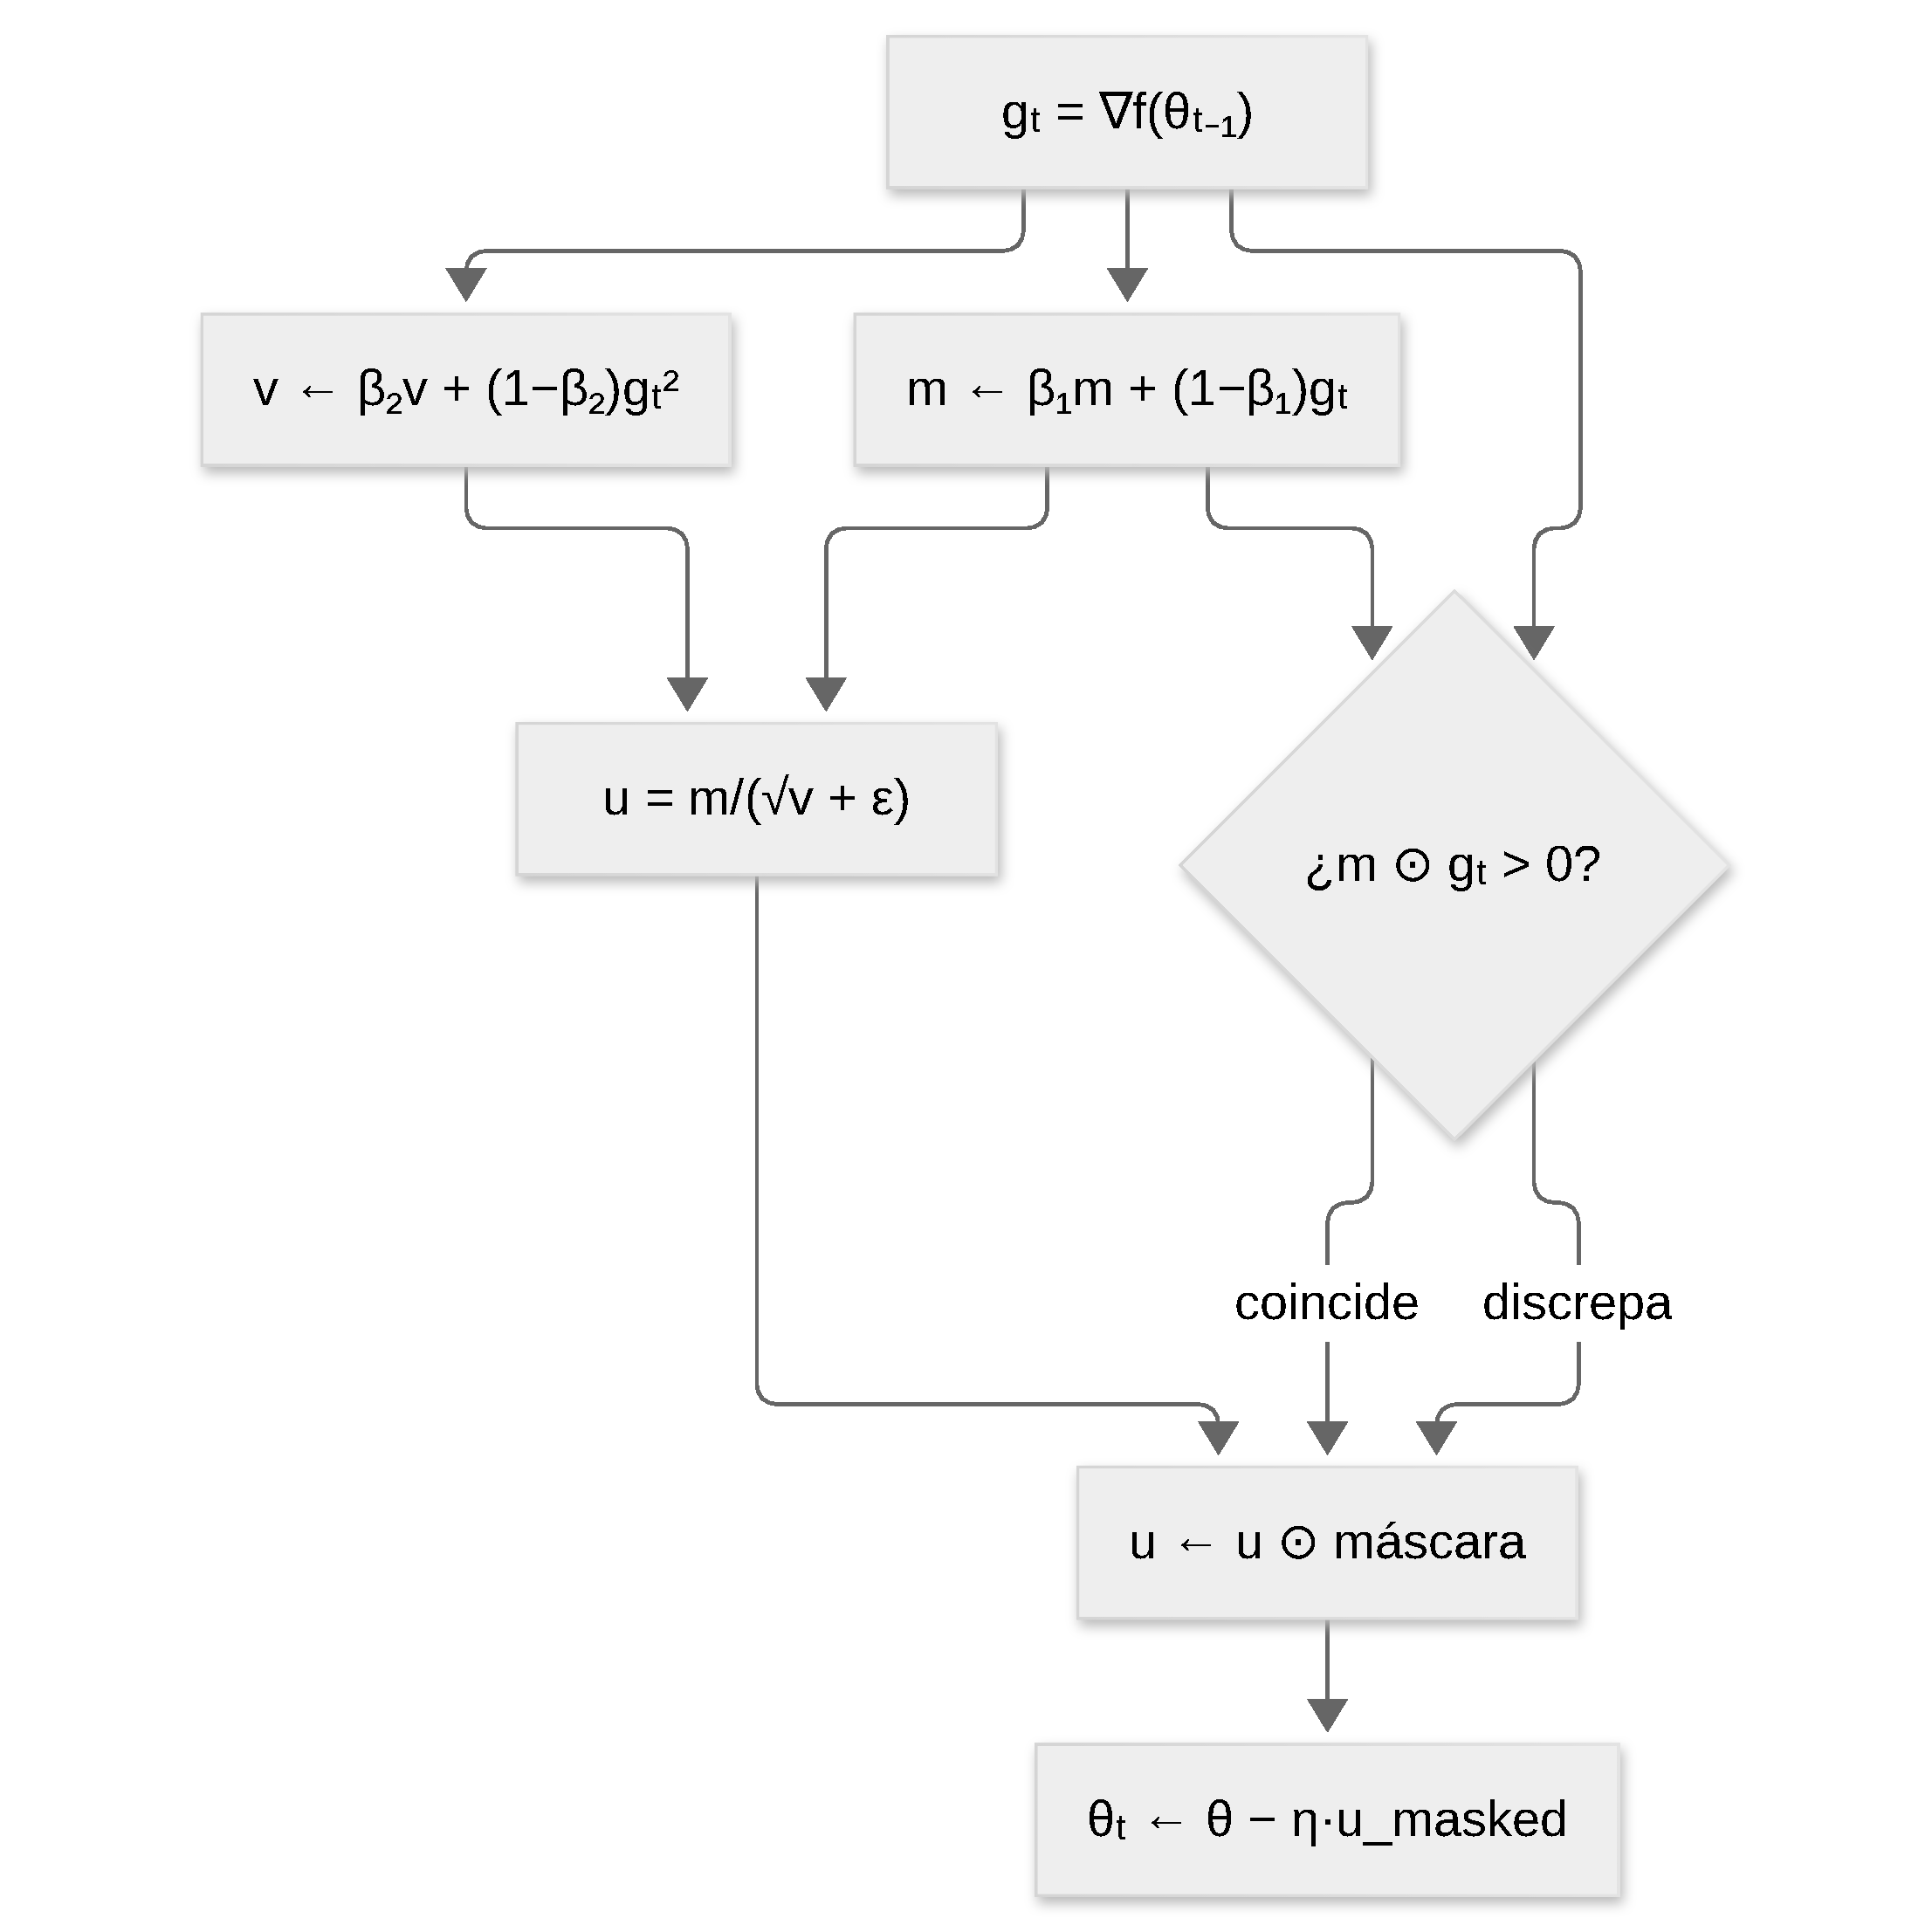
\includegraphics{../paper/figures/optimizers/cautious-es.pdf}}
\caption{Flujo por paso de Cautious AdamW: una máscara de consenso conserva solo las coordenadas donde momentum y gradiente coinciden.}
\label{fig:opt-cautious}
\end{figure}
El marco Cauteloso aplica una \textbf{modificación de una línea} a cualquier optimizador basado en momentum: enmascarar la actualización de modo que solo se apliquen las dimensiones donde el momentum y la dirección del gradiente coinciden:
\begin{align}
\text{mask}_i &= \begin{cases} 1 & \text{si } m_t[i] \cdot g_t[i] > 0 \quad\text{(acuerdo)} \\ 0 & \text{en caso contrario} \end{cases} \\
u_t &= \left(\frac{m_t}{\sqrt{v_t}+\epsilon}\right) \odot \text{mask} \quad\text{(enmascaramiento elemento a elemento)} \\
\theta_{t+1} &= \theta_t - \eta u_t
\end{align}
La intuición: el momentum $m_t$ estima la dirección del gradiente a partir del historial; el gradiente actual $g_t$ es la señal instantánea. Cuando ambos coinciden, el optimizador está seguro y debe actualizar agresivamente. Cuando discrepan, el optimizador está en conflicto---la tendencia histórica apunta hacia una región que pudo haber sido buena antes, pero la evidencia actual la contradice. Al enmascarar las dimensiones en conflicto, Cauteloso se vuelve más conservador y evita pasos corruptos.

\begin{algorithm}[H]
\caption{Cautious AdamW (Enmascaramiento de Actualización por Consenso)}
\label{alg:cautious}
\begin{algorithmic}[1]
\Require Parámetros iniciales $\theta_0$, tasa de aprendizaje $\eta$, $\beta_1, \beta_2$, decadencia de peso $\lambda$
\Ensure Parámetros actualizados $\theta_T$
\State Inicializar: $m \gets 0$, $v \gets 0$
\For{$t = 1, 2, \ldots, T$}
    \State $g_t \gets \nabla f(\theta_{t-1})$
    \State $m \gets \beta_1 m + (1-\beta_1) g_t$
    \State $v \gets \beta_2 v + (1-\beta_2) g_t^2$
    \State Máscara de consenso: $\text{mask}_i \gets 1$ si $m[i] \cdot g_t[i] > 0$, si no $0$ \Comment{Acuerdo}
    \State Actualización base Adam: $u \gets m / (\sqrt{v} + \epsilon)$
    \State Aplicar máscara: $u_{\text{masked}} \gets u \odot \text{mask}$ \Comment{Elemento a elemento}
    \If{decadencia\_de\_peso $> 0$}
        \State $\theta_{t-1} \gets \theta_{t-1}(1 - \eta\lambda)$
    \EndIf
    \State $\theta_t \gets \theta_{t-1} - \eta u_{\text{masked}}$
\EndFor
\Return $\theta_T$
\end{algorithmic}
\end{algorithm}

\paragraph{Contras.}
\begin{itemize}[leftmargin=*]
\item El enmascaramiento puede descartar actualizaciones útiles cuando momentum y gradiente discrepan temporalmente.
\item Requiere un optimizador base con momentum además de la máscara elemento a elemento.
\end{itemize}

\paragraph{Ventajas.}
\begin{itemize}[leftmargin=*]
\item Modificación de una línea aplicable a cualquier optimizador basado en momentum.
\item Hasta \textbf{1.47$\times$ de aceleración} en el preentrenamiento de Llama y MAE preservando las garantías de convergencia.
\end{itemize}

